\documentclass{scrartcl}
\usepackage[utf8]{inputenc}
\usepackage[UKenglish]{babel}
\usepackage{caption}
\usepackage{listings}
\usepackage{pdfpages}
\usepackage{amsmath}

\lstset{frame=single,keepspaces=true,captionpos=b}

\title{Homework 01 - kNN \& Decision Trees}
\author{Arne Sachtler - \textit{Registration Number: 03692662}}
\date{\today}
\subtitle{IN2064 Machine Learning}

\begin{document}
\maketitle
	
\section{Problem 1}
The tree is built automatically by a written python script. It prints the resulting tree by a textual description:
\lstinputlisting[caption={Final decision tree generated from the given exemplary data with a maximum depth of two.}]{tree_text}

Generating a set of artificial test data and using the generated decision tree in order to predict the class of the generated test data reveals the learned class decision as shown in Figure~\ref{fig:tree}.

\begin{figure}[h]
	\centering
	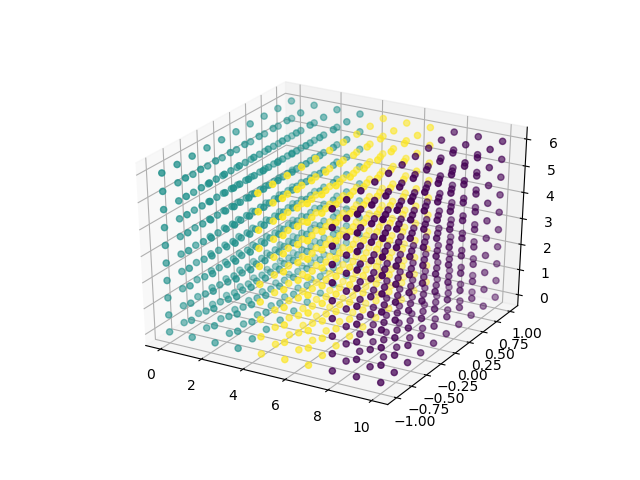
\includegraphics[height=5cm]{figure_tree.png}
	\caption{Class prediction for artificially generated test data.}
	\label{fig:tree}
\end{figure}

\section{Problem 2}
The following table summarises the predicted classes for the two given data points.

\begin{table}[h]
	\centering

	\begin{tabular}{l|c|c}
	\hline

	\hline
	\textbf{Data Point} $\mathbf{x}$ & \textbf{Predicted Class} $y$ & \textbf{Probability} $p(c = y | \mathbf{x}, T)$\\
	\hline
		 $\mathbf{x_a} = \begin{pmatrix}
		 	4.1 & -0.1 & 2.2
		 \end{pmatrix}^\top$& $y_a = 1$ & $p(c = y_a | \mathbf{x}_a, T) = 100\% $\\
	\hline
		$\mathbf{x_b} = \begin{pmatrix}
			6.1 & 0.4 & 1.3
		\end{pmatrix}^\top$ & $y_b = 2$ & $p(c = y_b | \mathbf{x}_b, T) = 66.6\% $\\

	\hline
	\end{tabular}
	\caption{Predicted classes for the given data points by the learned decision tree.}
	\label{tab:class_predictions}
\end{table}

\section{Problem 3}
See the pdf pages attached.

\section{Problem 4}
\section{Problem 5}
\section{Problem 6}

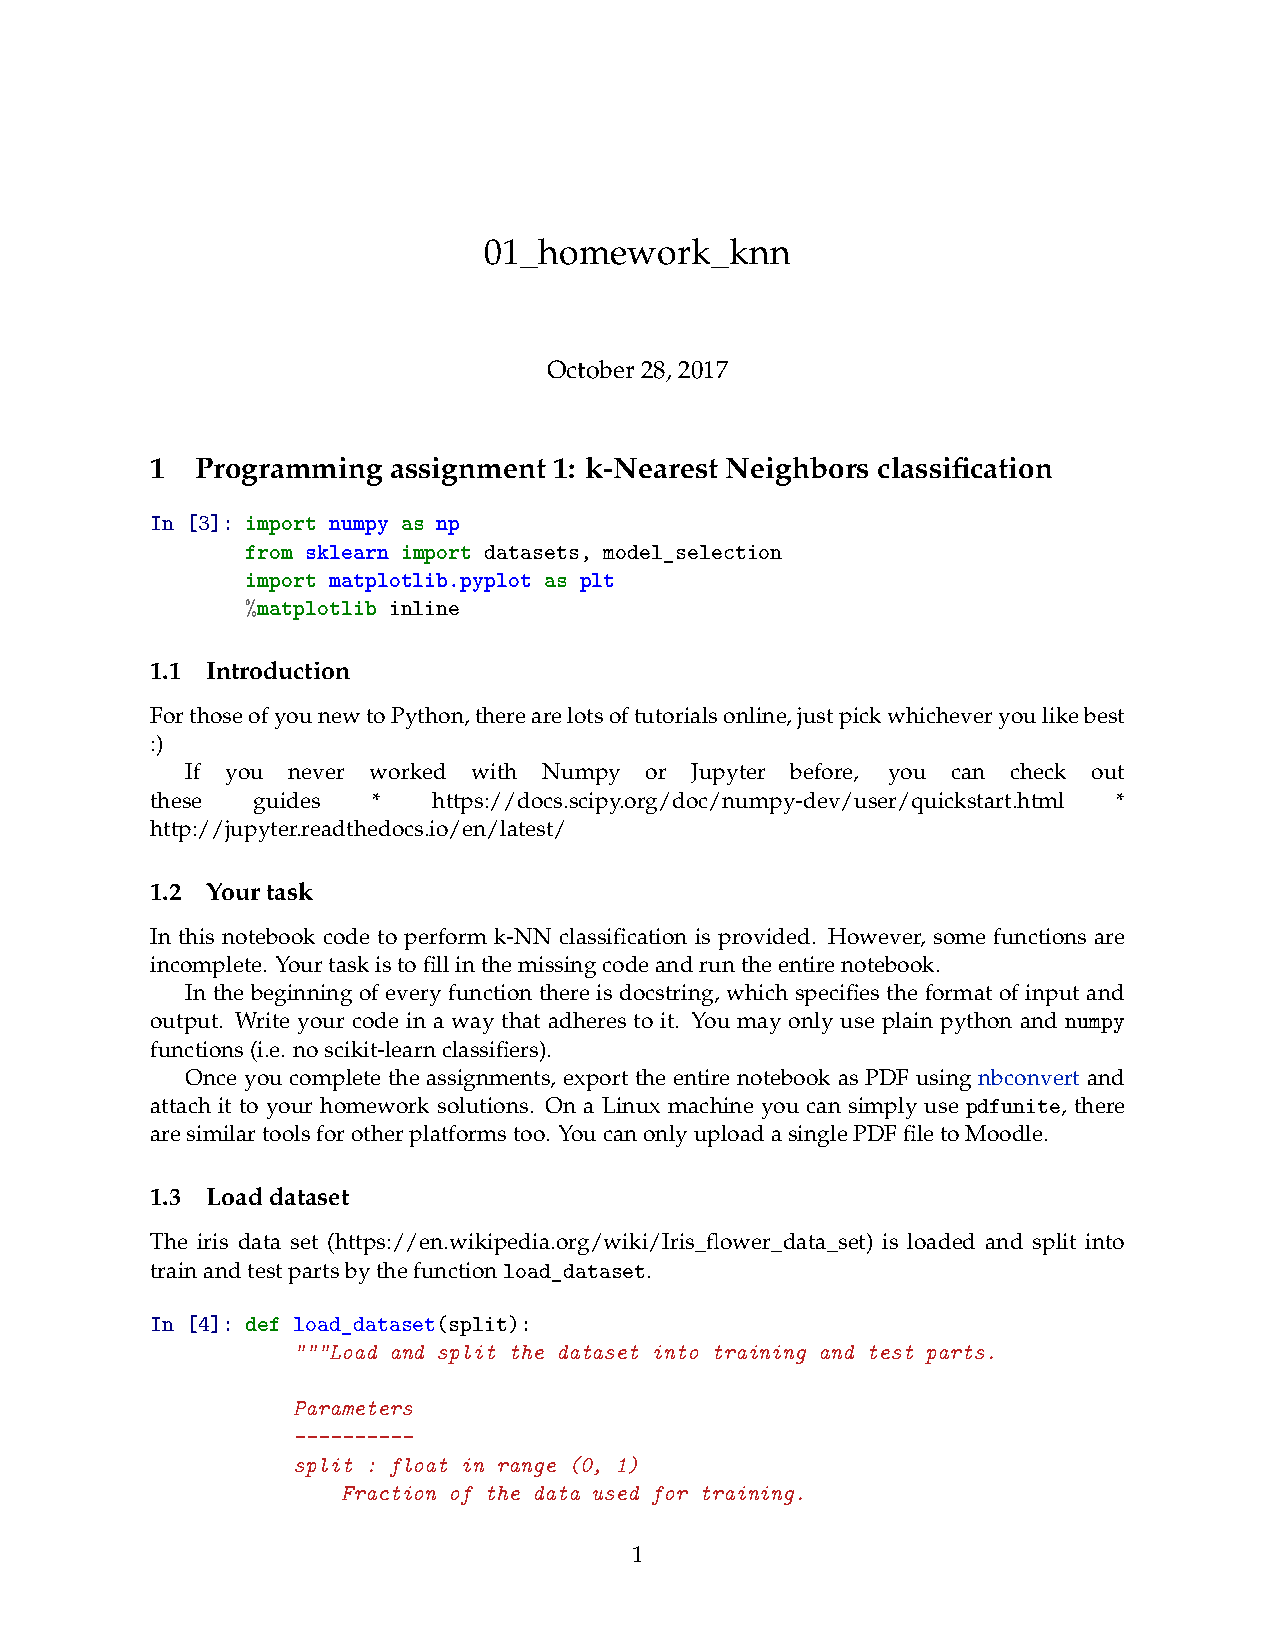
\includepdf[pages=-]{01_homework_knn.pdf}

\end{document}